% ---------------------------------------------------------------------
% EG author guidelines plus sample file for EG publication using LaTeX2e input
% D.Fellner, v2.02, Jan 25, 2017


\title[Seminar Topic]%
      {Graph Layouting for Visualizing Graph Structured Data}

% for anonymous conference submission please enter your SUBMISSION ID
% instead of the author's name (and leave the affiliation blank) !!
\author[M.Rosier \& K.\"ohlein]
{\parbox{\textwidth}{\centering Marcel Rosier$^1$% 
\\ Seminar: Data Visualization %
\\ marcel.rosier@tum.de% 
\\ Supervisor: Kevin H\"ohlein%
%        S. Spencer$^2$\thanks{Chairman Siggraph Publications Board}
        }
        \\
% For Computer Graphics Forum: Please use the abbreviation of your first name.
{\parbox{\textwidth}{\centering $^1$ Technische Universit\"at M\"unchen
%        $^2$ Another Department to illustrate the use in papers from authors
%             with different affiliations
       }
}
}
% ------------------------------------------------------------------------

% if the Editors-in-Chief have given you the data, you may uncomment
% the following five lines and insert it here
%
% \volume{36}   % the volume in which the issue will be published;
% \issue{1}     % the issue number of the publication
% \pStartPage{1}      % set starting page
\[\]

%-------------------------------------------------------------------------
\begin{document}

\teaser{
 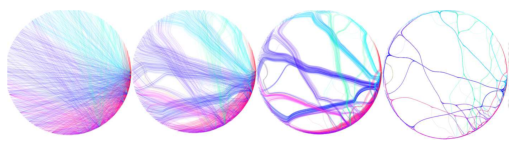
\includegraphics[width=\linewidth]{media/example_teaser.pdf}
 \centering
  \caption{Edge Bundling teaser, currently just a placeholder, modified from \cite{Lhuillier2017}}
\label{fig:teaser}
}

\maketitle
%-------------------------------------------------------------------------
\begin{abstract}
   TODO
   
%-------------------------------------------------------------------------
%  ACM CCS 1998
%  (see http://www.acm.org/about/class/1998)
% \begin{classification} % according to http:http://www.acm.org/about/class/1998
% \CCScat{Computer Graphics}{I.3.3}{Picture/Image Generation}{Line and curve generation}
% \end{classification}
%-------------------------------------------------------------------------


\end{abstract}  
%-------------------------------------------------------------------------
\section{Introduction}
A graph is mathematically defined as a tuple $ G = (V, E)$ with $V$ being a set of vertices (often also referred to as nodes) and $E \subseteq V^2$ being a set of edges \cite{Al-Taie2017}.[Graphs are used for representation of data, bridge from pure math to data vis.] Each edge describes a relation between two nodes and can be either directed or undirected. A sequence of edges along distinct vertices is called a path. Moreover Edges and vertices can have attributes, that provide additional information about them. Graphs can also be time dependent and modifiable, e.g. through user interaction. These graphs are called dynamic. Due to the scope of this paper only static graphs will be considered. 
\\\\
% Graphs come in various forms: Reaching from simple hierarchical Trees, e.g. in a file system, to gigantic graphs with millions of nodes and edges, for instance a social network.
In various areas - such as Biology, Software Engineering or the analysis of Social Networks - graphs are a typical way of representing data. In order to analyze the stored information, it is necessary to visualize it. Therefore the mathematical concept of a graph needs to be mapped to a visual representation. This process isn't trivial since except for special cases like geographic data vertices have no fixed position.
The procedure of mapping a graph to a usually 2 or 3 dimensional area is called graph layouting. 
Considering the size of typical graphs that can quickly exceed thousands of nodes and edges - for example a graph representing a social network like Facebook -  the layout of a graph has a huge impact on understanding the local and global structure, connections and other analysis tasks. Thus layout techniques try to maximize readability by taking different aesthetic criteria into account. To further improve readability the graph can be reduced in its complexity. Typical methods are for instance filtering, grouping or edge bundling (e.g. \autoref{fig:teaser}) which can be applied algorithmically, by a user or combined. \\ This paper is organized as follows: Section 2 gives an overview of possible visual representations of a graph and different families of layouting algorithms. In Section 3 state of the art complexity reduction strategies are explained with a heavy focus on edge bundling techniques and section 4 outlines common user interaction methods. Finally Section 5 summarizes the main aspects and points to open research topics.


\section{Visual Representation}
\subsection{Visualization options and criteria}
Graph Visualizations usually come in two types: node-link diagrams and adjacency matrices.
Node-link diagrams map vertices to items and edges to links between the items. Positioning the nodes and drawing the links in an appropriate way, e.g. minimize edge crossings, is challenging. Adjacency matrices on the other side have no issues with edge crossings. In this approach a graph with $N$ vertices is visualized by a $N * N $ matrix, in which every entry represents the edge between the vertices of the corresponding row and column. To optimize readability an optimal node order has to be calculated, the edges are then implicitly displayed.
Both types have certain benefits: In a direct comparison node-link diagrams are more intuitive, compact and make it easier to follow paths but can be hard to understand due to problematic layouts. Adjacency matrices provide an uncluttered view for dense graphs but have issues displaying large networks \cite{Ghoniem2004}. Some approaches also combine the 2 types to synthesize their advantages. Examples for all mentioned options can be found in \autoref{fig:vis_types}.
% This representation provides an intuitive overview and allows users to easily follow paths \cite{}
\\
\\
\begin{figure}
    \centering
    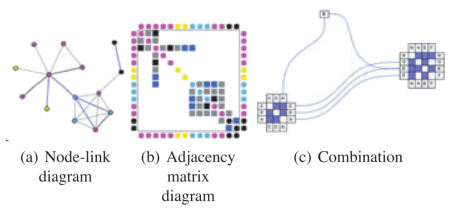
\includegraphics[width=\linewidth]{media/vis_types.pdf}
    \caption{bad quality -> improve and adapt or find other figure; \cite{VonLandesberger2011}}
    \label{fig:vis_types}
\end{figure}


\begin{itemize}
    \item whats a good layout? aesthetic criteria 
\end{itemize}

\subsection{Layout Techniques}
\begin{itemize}
    \item algorithms for special graph types: e.g. trees 
    \item force based families
    \item constraint based
    \item multi-scale approaches
    \item Non standard layouts: e.g. dimension reduction
\end{itemize}

\section{Complexity Reduction}

\subsection{Preprocessing}
Filtering and aggregation
\subsection{Grouping/ Clustering}

\subsection{Edge Bundling}
Explain the core idea of edge bundling and different methods
\begin{itemize}
    \item Techniques/ Methods
    \item Visualizations: Blending, Data color mapping, Shading, Smoothing and Deformation
    \item Discussion: Pro/con, mention its possible that non existent patterns are recognized
\end{itemize}

\section{User Interaction}
\begin{itemize}
    \item Panning, Zooming
    \item Magic Lense, Fisheye, Focus+context
    \item Adapt visualization parameters
\end{itemize}

\section{Conclusions}
Citations so they show up in the references:
\cite{Herman2000}
\cite{VonLandesberger2011}
\cite{Goyal2018}
\cite{Lhuillier2017}
\cite{Vehlow2015}
\cite{Gibson2013} \\


%-------------------------------------------------------------------------

%\bibliographystyle{eg-alpha}
\bibliographystyle{eg-alpha-doi}

\bibliography{references}

%-------------------------------------------------------------------------


\end{document}

